\subsection{Uncertainties in gas chemistry}
\label{sec:uncergaschem}
Prior studies have shown that the predicted concentrations of large PAHs can vary by orders of magnitude depending on the reaction mechanism used~\citep{wang2023systematic}. This variation introduces substantial uncertainty in the predicted rates of soot inception and surface growth. As a result, the reliability of soot simulations depends more on the accuracy of upstream chemical kinetics than on the rate constants of the inception models.

To illustrate the impact of chemical mechanism selection on predict soot properties, a series of simulations\footnote{\href{https://github.com/mohammadadib-cu/omnisoot-cv/tree/main/examples/pressure/mechanism_comparison}{https://github.com/mohammadadib-cu/omnisoot-cv/tree/main/examples/pressure/mechanism\_comparison}} were performed using the CPR model of Omnisoot (with soot formation disabled) for the pyrolysis of 5\%~$\mathrm{CH_4}$-Ar mixture at $\mathrm{T_5}=2203$~K and $\mathrm{P_5}=4.9$~atm~\citep{clark2025}. Six widely used chemical mechanisms were evaluated: ABF~\citep{appel2000kinetic}, Caltech~\citep{blanquart2009chemical}, KAUST~\citep{wang2013pah}, CRECK~\citep{saggese2015kinetic}, ITV~\citep{hellmuth2024role}, and FFCM2~\citep{ZDV2023}.

Fig.~\ref{fig:CH4_C2H2_C2H4_chem} shows the large variability in the predicted mole fraction of $\mathrm{CH_4}$, $\mathrm{C_2H_4}$, and $\mathrm{C_2H_2}$ across different reaction mechanisms. The mole fraction of $\mathrm{CH_4}$ serves as a useful indicator of carbon flux from the fuel to small and large intermediates. The CRECK and KAUST mechanisms significantly underpredict methane mole fraction compared to the measurements, but ABF and FFCM2 provide more accurate prediction considering the uncertainty of the experimental data.  The carbon flux analysis by \citet{wang2023systematic} highlighted the major role of C$_2$H$_4$ in the production of C$_2$H$_2$ via vinyl radical (C$_2$H$_3$). The overall trend of C$_2$H$_4$ mole fraction is captured by all mechanisms. After the rapid initial jump, C$_2$H$_4$ reaches its peak, which is underpredicted by ITV and overpredicted by KAUST. The subsequent decline was overestimated by all mechanisms that predict the final value of $\simeq$10$^{-4}$ below the measurements. A similar variability is observed in the prediction of $\mathrm{C_2H_2}$ mole fraction: it is best captured by FFCM2, overpredicted by CRECK, and slightly underpredicted by the ITV and Caltech mechanisms. Among all, FFCM2 shows the best overall agreement with the measurements; however, this mechanism only includes $\mathrm{C_1}$-$\mathrm{C_4}$ species and excludes benzene and larger PAHs, so it cannot be coupled with the soot models considered in this study.
\begin{figure}[!t]
	\centering
	\begin{tikzpicture}
		\draw (0, 0) node[inner sep=0] 	{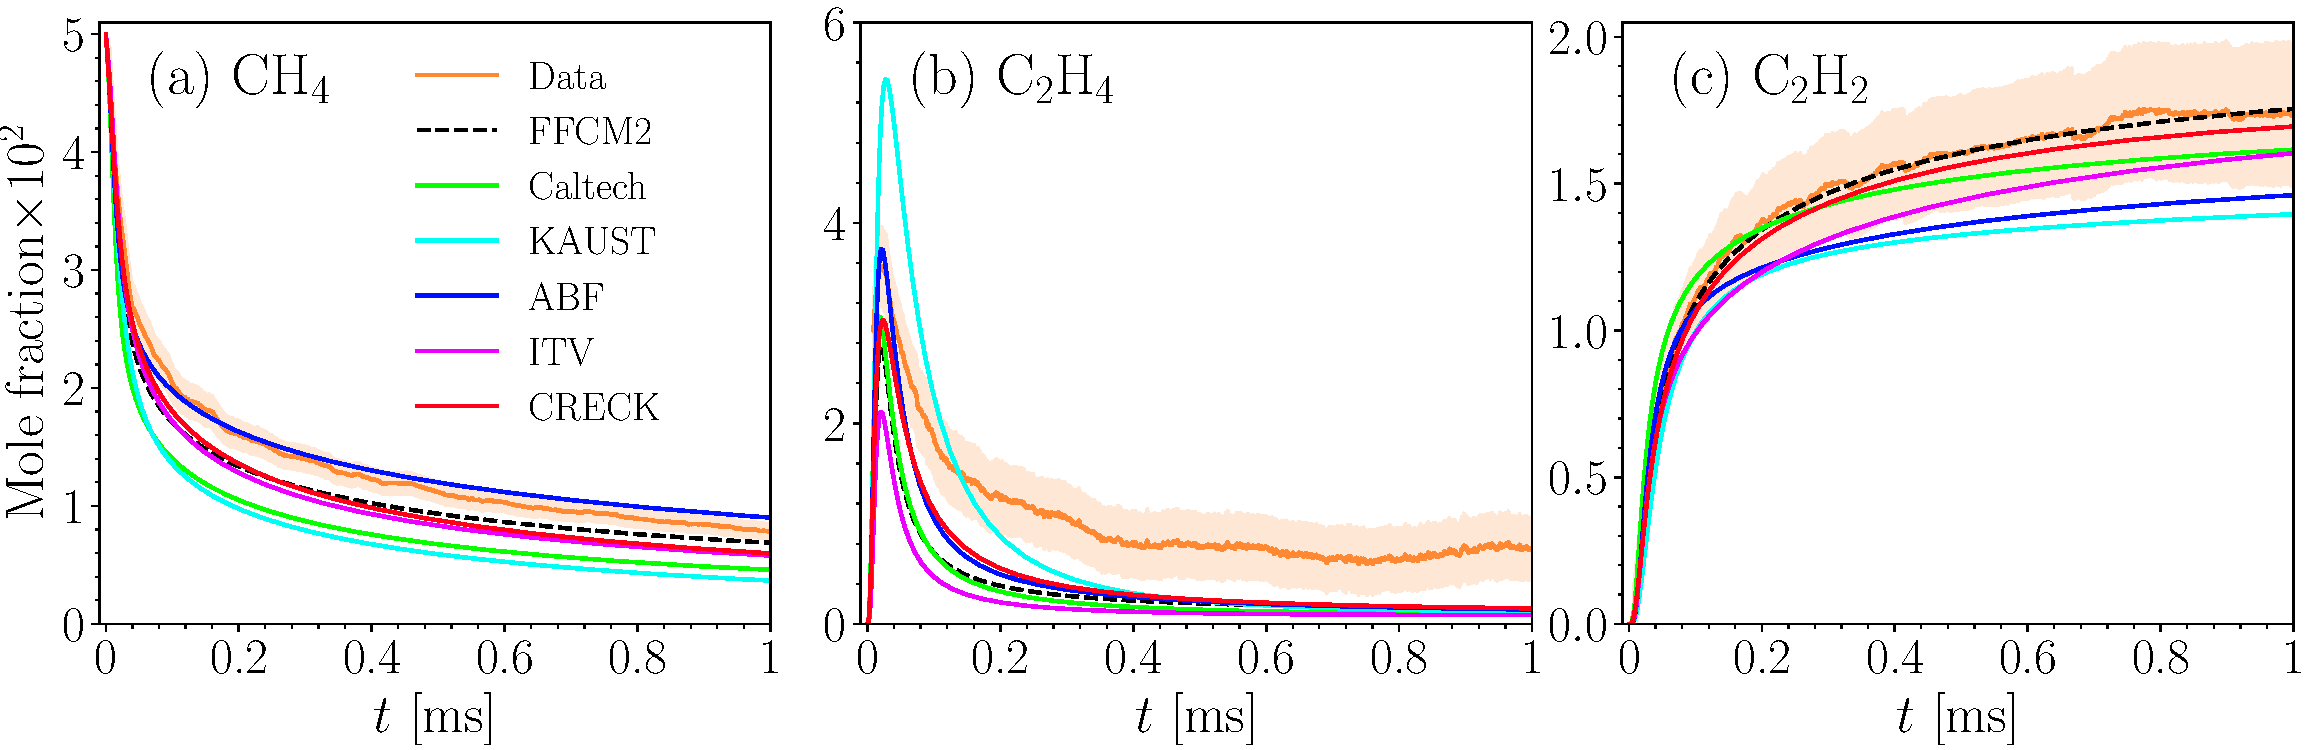
\includegraphics[width=1\textwidth]{Figures/Results/Paper1/chemistry/CH4_C2H4_C2H2.pdf}};
		\draw (-0.4, 1.93) node {\scriptsize{\citep{clark2025}}};
	\end{tikzpicture}
	\caption{The mole fraction of $\mathrm{CH_4}$ (a), $\mathrm{C_2H_4}$ and $\mathrm{C_2H_2}$ (c) during pyrolysis of 5\%~$\mathrm{CH_4}$-Ar predicted using different reaction mechanisms and compared with measurements~\citep{clark2025}.}
	\label{fig:CH4_C2H2_C2H4_chem} 
\end{figure}

\begin{figure}[!t]
	\centering
	\begin{tikzpicture}
		\draw (0, 0) node[inner sep=0] 	{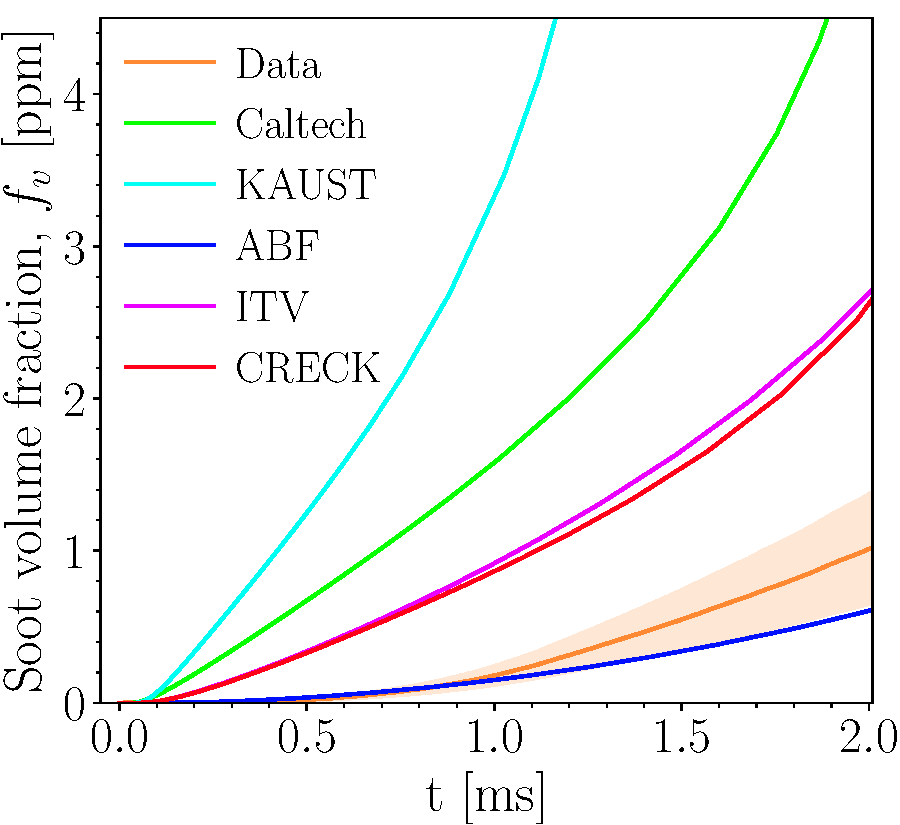
\includegraphics[width=0.38\textwidth]{Figures/Results/Paper1/chemistry/soot_fv_max.pdf}};
		\draw (-0.48, 2.0) node {\scriptsize{\citep{clack2025}}};
	\end{tikzpicture}
	\caption{The maximum soot volume fraction predicted using Irreversible Dimerization and different reaction mechanisms during pyrolysis of 5\%~$\mathrm{CH_4}$-Ar was compared with measurements~\citep{clark2025}. The shaded area represents the uncertainty in the reported experimental data.}
	\label{fig:max_sootfv_chem} 
\end{figure}


Next, we examine the maximum possible soot yield predicted by the selected mechanisms (excluding FFCM2) during 5\% $\mathrm{CH_4}$ pyrolysis at $\mathrm{T_5} = 2203$~K and $\mathrm{P_5} = 4.9$~atm. To do so, the Irreversible Dimerization model is employed with 100\% efficiency for both inception and PAH adsorption (i.e., all collisions lead to inception or surface growth). As shown in Fig.~\ref{fig:max_sootfv_chem}, the maximum possible $f_v$ predicted by the mechanisms shows greater relative variation than that observed for $\mathrm{CH_4}$ and $\mathrm{C_2H_2}$. Furthermore, the $f_v$ predicted by the ABF mechanism is lower than the measured value, even when accounting for the reported uncertainty. The same analysis was performed for other data points with a different $\mathrm{T_5}$ in~\citep{clark2025}, and similar results were observed indicating that ABF mechanism cannot provide enough precursors under pyrolysis conditions in these simulations. In contrast, the maximum possible $f_v$ predicted by other mechanisms is significantly larger than the measurements, which presents the possibility of predicting $f_v$ close to the measurements using more realistic assumptions (i.e., lower dimerization efficiencies). Caltech and KAUST mechanisms are used in the simulations of this study for description of gas chemistry as they provide the highest carbon flux to soot precursors, and they are still computationally more affordable than ITV and CRECK mechanisms for parametric studies.

In the rest of the results, the inception and PAH adsorption rates of PAH growth models are adjusted by calibrating $\eta_{inc}$ and $\eta_{ads}$ to match predict soot properties with available measurements. Note that, this approach does not resolve the mechanistic uncertainties of soot formation. Instead, it allows the model to calculate effective carbon fluxes from the gas phase into the particle phase that are consistent with measured soot properties. Our analysis showed that all PAH growth models require different sets of $\eta_{inc}$ and $\eta_{ads}$ to capture the measured soot properties in the studied conditions. The lack of universal factors highlights the uncertainties in concentration of gaseous species, potential missing inception and surface growth pathways, and unknown sensitivities to temperature and fuel composition.